\documentclass[10pt, hyperref={bookmarks=false}, show notes]{beamer}
% Text
        \usepackage[T1]{fontenc}
        \usepackage[utf8]{inputenc}
        \usepackage[english]{babel}
        \usepackage[bitstream-charter]{mathdesign} % Serif font (Charter BT).
        \usepackage[scaled=0.84]{DejaVuSansMono} % Monospaced font.
        \def\sfdefault{SourceSansPro-TLF} % Sans serif font.
        \usepackage{textcomp}

% Maths
  \usepackage{amsmath}
  \usepackage{mathtools}
  \usepackage{siunitx}
  % Vector command
  \newcommand{\omatrix}[1]{\ensuremath{\boldsymbol{#1}}}

% Graphics
  \usepackage{graphicx}
  \usepackage[caption=false]{subfig}
        \usepackage{tikz}
  \usepackage{pgfplots}
  \pgfplotsset{compat=1.10}
        % ADD TIKZ LIBRARIES
  \usetikzlibrary{calc}
  \usetikzlibrary{arrows.meta}
  \usepackage{tikz-qtree}
  \usetikzlibrary{decorations.pathmorphing}
  \usetikzlibrary{matrix,shapes,positioning,fit}
  \usepgfplotslibrary{external}
  \tikzexternalize[prefix=graphics/tikz/]
  \tikzexternaldisable % Disable by default
  \usepackage{tabularx}
  \usepackage{pgfgantt}
  \usepackage{multirow}
  \usepackage{hhline}

        \usepackage{xcolor}
    \definecolor{color1}{cmyk}{100,50,0,0}   % blue
    \definecolor{color2}{cmyk}{0,80,100,0}   % vermillion
    \definecolor{color3}{cmyk}{97,0,75,0}    % blueish green
    \definecolor{color4}{RGB}{204,121,167}    % reddish purple
    \definecolor{color5}{RGB}{230,159,0}   % orange
   \usepackage{colortbl}
% Misc
\usepackage{booktabs}
\usepackage{enumerate}
\usepackage{pdfpages}
\usepackage{pgfpages}
\usepackage{setspace}
\usepackage{adjustbox}
%\usepackage{multimedia}

\setbeamertemplate{navigation symbols}{}
\setbeamertemplate{caption}{\raggedright\insertcaption\par}
%\setbeamertemplate{bibliography item}[text]

\usepackage{caption}
\usetheme{/amsterdam}
\date

\usepackage{beamertheme/handoutWithNotes}
% Uncomment for handouts. Add \documentclass[12pt,handout]{beamer}
%\pgfpagesuselayout{4 on 1 with notes}[a4paper,border shrink=5mm]
% Comment for handouts.
%\setbeameroption{show notes on second screen=right}

% Table of content dybde (0-index)
%\setcounter{tocdepth}{1}

% BibLaTeX
%\usepackage{csquotes}
%\usepackage[
%backend=bibtex,
%citestyle=numeric,
%bibstyle=numeric,
%maxcitenames=3,
%maxbibnames=99,
%url=true]{biblatex}
%\addbibresource{../rapport/references/refs.bib}
%\addbibresource{extrasources.bib}
%\usepackage{../style/biblatex_custom_formatting}

\graphicspath{{graphics/}{../../Report/graphics/}}

\begin{document}

%\captionsetup[figure]{font=small,singlelinecheck=off,justification=raggedright}

\title[Group Recommender Using Voting as Mediator]{TrashVision}
\author[\insertframenumber /\inserttotalframenumber]{Claus N. Madsen, Lasse D. Christensen, Lukas N. Dalgaard}

\begin{frame}
\Large Group Recommender Using Voting as Mediator\\
\small Claus N. Madsen, Lasse D. Christensen, Lukas N. Dalgaard\\
\end{frame}

\begin{frame}
  \frametitle{Contents}
  \tableofcontents
  \note{
  \begin{itemize}
    \item Scenario 
    \item Novel rank aggregation 
    \item Evaluation methodology
    \item Results 
    \item Conclusion 
    \item Future work
  \end{itemize}
}
\end{frame}

% PUT INPUTS HERE
\section{Scenarios}

\subsection{Group Movie watching}
Size: 3-6
Group needs to decide on a movie to watch. They are able discuss it among themselves. The people do not necessarily know each other, but they are likely friends or acquaintances.
\subsection{Gathering with Music}
size: 3-6
Group needs to decide on the sequence of music playing. There are few enough that a sort of consensus could be reached via dialog. All within hearing distance of each other. The people do not necessarily know each other, but they are likely friends or acquaintances.
\subsection{Party with Music}
size: 20-100
Group needs to decide on the sequence of music playing. They are able to communicate, however from the size and context of the event, it is impractical as the focus is elsewhere for most people to quickly reach a consensus. There are likely clusters of friends, however the group is more randomly put together.
\section{Novel Aggregation Methods} \label{sec:novelaggregationmethods}
In this section new aggregation methods are presented. The methods are described and exemplified using the small randomly generated dataset seen in Table \ref{tbl:randomratingstable}.

\begin{table}[H]
	\centering
	\begin{tabular}{|l|l|l|l|l|l|l|l|l|l|l|}
		\hline
		& T1  & T2  & T3  & T4  & T5  & T6  & T7  & T8  & T9  & T10 \\ \hline
		U1 & 1.2 & 2.9 & 3.0 & 5.0 & 1.0 & 1.7 & 4.1 & 5.0 & 4.9 & 4.0 \\ \hline
		U2 & 2.2 & 3.6 & 4.3 & 2.1 & 1.8 & 2.8 & 1.3 & 5.0 & 1.1 & 3.5 \\ \hline
		U3 & 1.9 & 2.7 & 1.6 & 3.9 & 4.3 & 1.7 & 1.2 & 1.9 & 4.5 & 4.4 \\ \hline
		U4 & 4.4 & 3.9 & 1.6 & 3.7 & 1.0 & 2.7 & 3.6 & 3.0 & 3.9 & 2.6 \\ \hline
		U5 & 2.3 & 3.5 & 4.6 & 3.5 & 3.4 & 3.0 & 4.5 & 4.7 & 3.0 & 3.9 \\ \hline
	\end{tabular}
	\caption{Randomized table of ratings for 5 users with 10 items.}
	\label{tbl:randomratingstable}
\end{table}


\begin{table}[H]
	\centering
	\begin{tabular}{|l|l|l|l|l|l|l|l|l|l|l|}
		\hline
		& T1 & T2 & T3 & T4 & T5 & T6 & T7 & T8 & T9 & T10 \\ \hline
		U1    & 2  & 4  & 5  & 9  & 1  & 3  & 7  & 9  & 8  & 6   \\ \hline
		U2    & 5  & 8  & 9  & 4  & 3  & 6  & 2  & 10 & 1  & 7   \\ \hline
		U3    & 4  & 6  & 2  & 7  & 8  & 3  & 1  & 4  & 10 & 9   \\ \hline
		U4    & 10 & 8  & 2  & 7  & 1  & 4  & 6  & 5  & 8  & 3   \\ \hline
		U5    & 1  & 5  & 9  & 5  & 4  & 2  & 8  & 10 & 2  & 7   \\ \hline
		Total & 22 & 31 & 27 & 32 & 17 & 18 & 24 & 38 & 29 & 32  \\ \hline
	\end{tabular}
	\caption{Borda Count results from the randomized example}
	\label{tbl:bordacount}
\end{table}

\subsection{Borda Weighted Count}
Using Borda Count(BC) as a base and adding a weight to the items based on the number of times they occur in the top-k lists would help increase the score of those items multiple users have rated high enough to get onto their top-k list. Our implementation will use a simplistic weight of adding 1 additional point to the final tally of the scores for each time they appeared in the top-k lists the group members produced. Depending on the size of $k$ it could very well be that the weighting factor should be changed as the weight used would have little influence when scores of more than 50 are handed out.

An example of how the scores from the random samples top-4, Table \ref{tbl:top4borda}, have influenced the ordering can be seen in Table \ref{tbl:novelscoresexample}. The order has not changed per say, number 1 and 2 is T8 and T9 respectively just as in BC, however Borda Weighted Count(BWC) gives a shared third place to T3, T4, and T10, whereas BC gave the third place to T3 and had T4 and T10 on a shared fourth place. 

\subsection{Borda Escalated Count}
Borda Escalated Count(BEC) is based on the idea that BC does not necessarily give enough distinction to the top of the top-k items. This method will increase the scores given by the normal BC by some amount based on where in the top-k list the item appear. Our implementation will split the top-k list into three parts, the upper part will receive an extra 3 points to all items, the items in the middle part will be given 1 extra point, while the lower part will receive no extra points.

The example of how the scores would be are again presented in Table \ref{tbl:novelscoresexample}. Here T10 is no longer amongst the four items scoring the highest, while the others are placed as in BWC.

\subsection{Borda Transferable Count} \label{BTC}
As it was determined in Section \ref{sec:stv}, STV was unsuitable as a selection process, but by modifying the voting we believe that the problems with using STV in recommender systems can be accounted for. The change proposed for Borda Transferable Count(BTC) is changing the single vote into a BC score, so instead of a user only having 1 vote on a top-10 list, they would have 55, the highest rated item with 10, second item with 9, etc.. This approach should allow for more reliable selection, as users no longer end up only voting on their own highest rated items. Of course this relies on at least a few overlaps between items on the top-k lists.

Here is a simplified example of how it will perform if it is used on the random sample with top-4, see Table \ref{tbl:top4borda} and giving the results seen in Table \ref{tbl:novelscoresexample}.

\begin{enumerate}
	\item Threshold calculated to be 12.5, but for simplicity it is set to 13.
	\item No candidate exceeds the threshold, so instead the current worst candidate T5 is eliminated, their votes transferred to their highest priority T9.
	\item T7 is now the next to be eliminated, 1 vote moved to T4 and 2 votes to T8, T8 is now locked in.
	\item T8 hit our simplified threshold without exceeding it so no votes are transferred further, instead T1 is the next to be eliminated, only one user voted on it but their secondary choice is split between T2 and T9 so 2 votes will be transferred to each.
	\item Next up is T10 being eliminated and going by the lists, U2 and U3 would instead give their 4 combined votes to T9, while U5 would give a single vote to T8, but as that candidate is already locked in the vote is instead transferred to T3, the secondary choice.
	\item T9 now exceeds the threshold and 3 votes have to be transferred to other choices. For sake of simplicity the votes are handed out for users to redistribute equally, so U1, U3, and U4 each get one vote to reassign, U1 and U3 both give it to T4, while U4 gives it to T2.
	\item Next T2 is eliminated and the votes distributed equally between T3 and T4.
	\item There are now only four candidates left for four seats, and going by the order they were locked in and then the number of votes they got the order would be T8, T9, T4, and then T3.
\end{enumerate}

The resulting ordering is again not too different from the ones seen before, however it has been definitively reduced to only four candidates. The random data most definitely favored T8 and T9 in these small examples, so the fact that they are solidly chosen as the first and second place is fitting. Third and fourth place has been switched in BTC compared to the other orderings, however they have generally been close in general. That being said, the ordering of the candidates throughout the process have a large impact on which candidates that gets eliminated, which leads to some inherent bias.

\begin{table}[H]
	\centering
	\begin{tabular}{|l|l|l|l|l|}
		\hline
		& Rank 1 & Rank 2  & Rank 3 & Rank 4  \\ \hline
		U1 & T4 (3) & T8 (3)  & T9 (2) & T7 (1)  \\ \hline
		U2 & T8 (4) & T3 (3)  & T2 (2) & T10 (1) \\ \hline
		U3 & T9 (4) & T10 (3) & T5 (2) & T4 (1)  \\ \hline
		U4 & T1 (4) & T2 (2)  & T9 (2) & T4 (1)  \\ \hline
		U5 & T8 (4) & T3 (3)  & T7 (2) & T10 (1) \\ \hline
	\end{tabular}
	\caption{Ranking of the top-4 items for each user from Table \ref{tbl:randomratingstable}, BC score in parenthesis}
	\label{tbl:top4borda}
\end{table}

\begin{table}[H]
	\centering
	\begin{tabular}{|l|l|l|l|l|l|l|l|l|l|}
		\hline
		& T1 & T2 & T3   & T4   & T5 & T7 & T8  & T9  & T10 \\ \hline
		Borda & 4  & 4  & 6    & 5    & 2  & 3  & 11  & 8   & 5   \\ \hline
		BWC   & 5  & 6  & 8    & 8    & 3  & 5  & 14  & 11  & 8   \\ \hline
		BEC   & 7  & 6  & 8    & 8    & 3  & 4  & 18  & 13  & 6   \\ \hline
		BTC   & -  & -  & 10.5 & 11.5 & -  & -  & 13* & 13* & -   \\ \hline
	\end{tabular}
	\caption{Scores from each method on top-4, in BTC the * indicates the candidate hitting the threshold}
	\label{tbl:novelscoresexample}
\end{table}
\section{Code Review}

\begin{frame}
     \begin{center}
     	\huge Code Review
     \end{center}
\end{frame}

\begin{frame}
	\frametitle{Problems}
	\begin{itemize}
		\item Error in implementation of the DCG and IDCG algorithm
	\end{itemize}

	\begin{equation}\label{eq:background_dcg}
	\text{(I)DCG}_p = \sum_{i=1}^{p}\frac{\textit{rel}_i}{\log_2(i + 1)}
	\end{equation}	
	
	\begin{itemize}
		\item Misconception of how to find the ideal list for IDCG
	\end{itemize}
	
	\begin{table}[h]
		\centering
		\begin{minipage}{.48\textwidth}\centering
			\begin{tabular}{|l|llll|}
				\hline
						& I1 & I4 & I3  & I2    \\ \hline
				James	& 4  & 3  & 2 	& 1	 	\\ \hline
			\end{tabular}
		\end{minipage}
		\hfill
		\begin{minipage}{.48\textwidth}\centering
			\begin{tabular}{|l|llll|}
				\hline
				Group	& I7 & I2 & I5  & I1    \\ \hline
			\end{tabular}
		\end{minipage}
	\end{table}
	
	\begin{table}[h]
		\begin{tabular}{|l|llll|}
			\hline
			Ideal from report	& I1 & I2 & I5  & I7    \\ \hline
			James score			& 4	 & 1  &	0	& 0		\\
			\hline
		\end{tabular}
	\end{table}
\end{frame}

%We have ratings for all users items, use these to determine satisfaction instead of just top-k.
%Use some average ordering of the top-k.
\section{Results}

\begin{frame}
     \begin{center}
     	\huge Results 
     \end{center}
\end{frame}

\begin{frame}
	\frametitle{Methodology}
	The setup of the new test is the same as the previous tests
	\begin{itemize}
		\item The exact same random generated groups as in the previous tests
		\item Groups of the sizes 4, 8, 12, 16, 20, and 40
		\item There are 1000 groups of each size
		\item The preferences looked at is the top 10
	\end{itemize}
\end{frame}

\begin{frame}
\frametitle{Group Size 4}
\begin{figure}[h]
\centering
\begin{minipage}{.46\textwidth}\centering
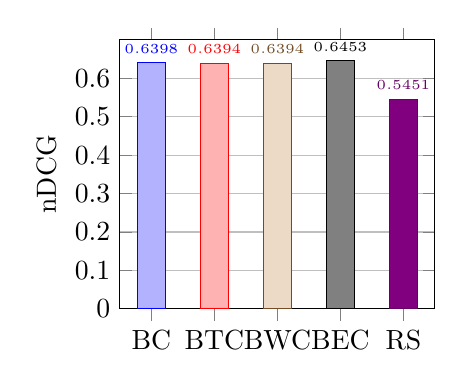
\begin{tikzpicture}
 \begin{axis}[
 	height=5cm,
 	width=4cm,
 	ybar =-10pt,
 	x = .8cm,
 	ymin=0.0, 
 	ymax=0.70,
 	ytick = {0, 0.1,0.2,0.3,...,0.70},
 	scaled y ticks = false,
	enlarge x limits ={abs=.4cm},
	nodes near coords,
    every node near coord/.append style={font=\tiny,/pgf/number format/.cd,precision=4},
 	ylabel={nDCG},
	xtick={0,1,2,3,4},  % NEW BIT
	xticklabels={BC, BTC, BWC, BEC, RS},
	%legend style={at={(0.5,-0.1)},
	%anchor=north,legend columns=-1},
	ymajorgrids = true,]

		\addplot coordinates {(0,0.6398)};    
		\addplot coordinates {(1,0.6394)};    
		\addplot coordinates {(2,0.6394)};    
		\addplot coordinates {(3,0.6453)};    
		\addplot coordinates {(4,0.5451)};
        %\legend{BC, BTC, BWC, BEC, Random}
     \end{axis}
\end{tikzpicture}
\end{minipage}
\begin{minipage}{.46\textwidth}\centering
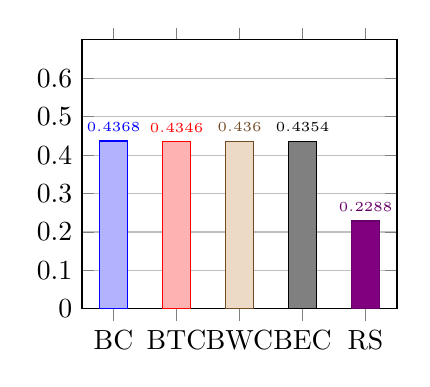
\begin{tikzpicture}
 \begin{axis}[
 	height=5cm,
 	ybar =-10pt,
 	x = .8cm,
 	ymin=0.0, 	
 	ymax=0.70,
 	ytick = {0,0.1,0.20,0.3,...,0.70},
	enlarge x limits ={abs=.4cm},
	nodes near coords,
    every node near coord/.append style={font=\tiny,/pgf/number format/.cd,precision=4},
	xtick={0,1,2,3,4},  % NEW BIT
	xticklabels={BC, BTC, BWC, BEC, RS},
	%legend style={at={(0.5,-0.1)},
	%anchor=north,legend columns=-1},
	ymajorgrids = true,]

		\addplot coordinates {(0,0.4368)};    
		\addplot coordinates {(1,0.4346)};    
		\addplot coordinates {(2,0.436)};    
		\addplot coordinates {(3,0.4354)};    
		\addplot coordinates {(4,0.2288)};
        %\legend{BC, BTC, BWC, BEC, Random}
     \end{axis}
\end{tikzpicture}
\end{minipage}
\end{figure}
\end{frame}

\begin{frame}
\frametitle{Group Size 12}
\begin{figure}[h]
\centering
\begin{minipage}{.46\textwidth}\centering
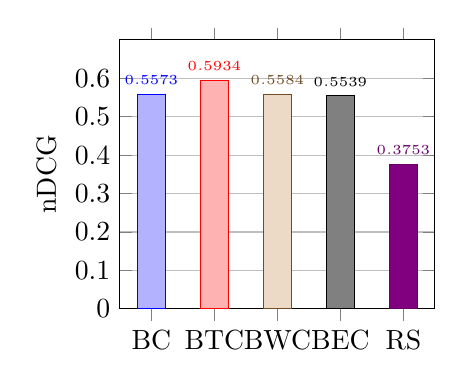
\begin{tikzpicture}
 \begin{axis}[
 	height=5cm,
 	width=4cm,
 	ybar =-10pt,
 	x = .8cm,
 	ymin=0.00, 
 	ymax=0.70,
 	ytick = {0,0.1,0.2,0.3,...,0.70},
 	scaled y ticks = false,
	enlarge x limits ={abs=.4cm},
	nodes near coords,
    every node near coord/.append style={font=\tiny,/pgf/number format/.cd,precision=4},
 	ylabel={nDCG},
	xtick={0,1,2,3,4},  % NEW BIT
	xticklabels={BC, BTC, BWC, BEC, RS},
	%legend style={at={(0.5,-0.1)},
	%anchor=north,legend columns=-1},
	ymajorgrids = true,]

		\addplot coordinates {(0,0.5573)};    
		\addplot coordinates {(1,0.5934)};    
		\addplot coordinates {(2,0.5584)};    
		\addplot coordinates {(3,0.5539)};    
		\addplot coordinates {(4,0.3753)};
        %\legend{BC, BTC, BWC, BEC, Random}
     \end{axis}
\end{tikzpicture}
\end{minipage}
\begin{minipage}{.46\textwidth}\centering
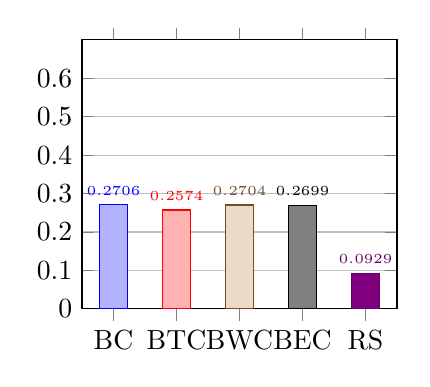
\begin{tikzpicture}
 \begin{axis}[
 	height=5cm,
 	ybar =-10pt,
 	x = .8cm,
 	ymin=0.0, 	
 	ymax=0.70,
 	ytick = {0,0.1,0.20,0.3,...,0.70},
	enlarge x limits ={abs=.4cm},
	nodes near coords,
    every node near coord/.append style={font=\tiny,/pgf/number format/.cd,precision=4},
	xtick={0,1,2,3,4},  % NEW BIT
	xticklabels={BC, BTC, BWC, BEC, RS},
	%legend style={at={(0.5,-0.1)},
	%anchor=north,legend columns=-1},
	ymajorgrids = true,]

		\addplot coordinates {(0,0.2706)};    
		\addplot coordinates {(1,0.2574)};    
		\addplot coordinates {(2,0.2704)};    
		\addplot coordinates {(3,0.2699)};    
		\addplot coordinates {(4,0.0929)};
        %\legend{BC, BTC, BWC, BEC, Random}
     \end{axis}
\end{tikzpicture}
\end{minipage}
\end{figure}
\end{frame}

\begin{frame}
\frametitle{Group Size 40}
\begin{figure}[h]
\centering
\begin{minipage}{.46\textwidth}\centering
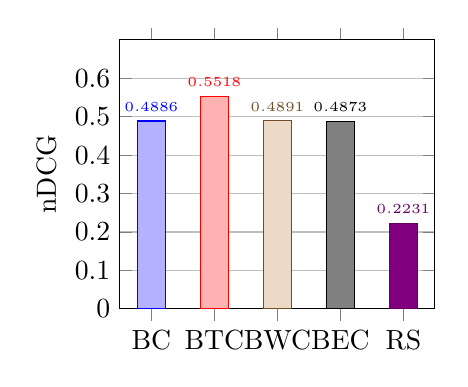
\begin{tikzpicture}
 \begin{axis}[
 	height=5cm,
 	width=4cm,
 	ybar =-10pt,
 	x = .8cm,
 	ymin=0.00, 
 	ymax=0.70,
 	ytick = {0,0.1,0.20,0.3,0.4,0.5,0.60},
 	scaled y ticks = false,
	enlarge x limits ={abs=.4cm},
	nodes near coords,
    every node near coord/.append style={font=\tiny,/pgf/number format/.cd,precision=4},
 	ylabel={nDCG},
	xtick={0,1,2,3,4},  % NEW BIT
	xticklabels={BC, BTC, BWC, BEC, RS},
	%legend style={at={(0.5,-0.1)},
	%anchor=north,legend columns=-1},
	ymajorgrids = true,]

		\addplot coordinates {(0,0.4886)};    
		\addplot coordinates {(1,0.5518)};    
		\addplot coordinates {(2,0.4891)};    
		\addplot coordinates {(3,0.4873)};    
		\addplot coordinates {(4,0.2231)};
        %\legend{BC, BTC, BWC, BEC, Random}
     \end{axis}
\end{tikzpicture}
\end{minipage}
\begin{minipage}{.46\textwidth}\centering
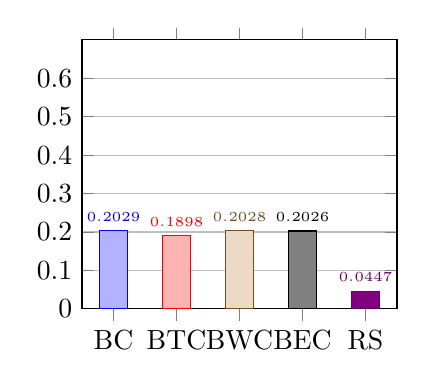
\begin{tikzpicture}
 \begin{axis}[
 	height=5cm,
 	ybar =-10pt,
 	x = .8cm,
 	ymin=0.0, 	
 	ymax=0.70,
 	ytick = {0,0.1,0.20,0.3,0.4,0.5,0.60},
	enlarge x limits ={abs=.4cm},
	nodes near coords,
    every node near coord/.append style={font=\tiny,/pgf/number format/.cd,precision=4},
	xtick={0,1,2,3,4},  % NEW BIT
	xticklabels={BC, BTC, BWC, BEC, RS},
	%legend style={at={(0.5,-0.1)},
	%anchor=north,legend columns=-1},
	ymajorgrids = true,]

		\addplot coordinates {(0,0.2029)};    
		\addplot coordinates {(1,0.1898)};    
		\addplot coordinates {(2,0.2028)};    
		\addplot coordinates {(3,0.2026)};    
		\addplot coordinates {(4,0.0447)};
        %\legend{BC, BTC, BWC, BEC, Random}
     \end{axis}
\end{tikzpicture}
\end{minipage}
\end{figure}
\end{frame}

\begin{frame}
	\frametitle{Possible Solutions}
	\begin{itemize}
		\item Calculate nDCG using the predicted ratings
		\item Ordering the individual ranked list by the average for the group
	\end{itemize}
\end{frame}
\subsection{Future Work}\label{sec:futurework}
%survey/Dataset 
%Context and influence 
%real world application
%Reordering of rank lists

\section*{}

\end{document}
